\documentclass{templateNote}
\usepackage{tcolorbox}
\usepackage{tabularx}
\usepackage{hyperref}
\usepackage{amsmath}
\usepackage{amssymb}
\usepackage{pdflscape}
\usepackage{tikz}
\usepackage{soul}
\usepackage{media9}
\usepackage{adjustbox}
\usepackage{pdfpages}
\usepackage{comment}
\usepackage{enumitem}
\usepackage{parskip}
% \usepackage[spanish,es-noquoting]{babel}

\begin{document}
\linklogoU{https://www.ubiobio.cl/w/}
\linklogoD{https://github.com/NicoGomezM}
\imagenlogoU{img/logo-ubb-txt-face.png}
\imagenlogoD{img/logoNGMFormal_sinF.png}
\titulo{Laboratorio 2: MiniShell}
\asignatura{Laboratorio Sistemas Operativos}
\autor{
    Nicolás \textsc{Gómez Morgado}
}

\portada
\margenes

% \section*{Ejercicios solicitados}

\section*{Ejercicios:}
\subsection*{Parte A}
\begin{enumerate}
    \item \& (5pts)
    \begin{figure}[H]
        \centering
        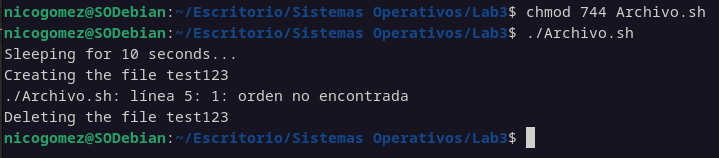
\includegraphics[width=\textwidth]{img/ejerc1.png}
        Se creo un archivo llamado \textit{Archivo.sh} en el cual se introdujo la secuencia de comandos asignada, como resultado se observa una correcta compilación a excepción de un error sintáctico en la línea 5, el cual se refiere a que hay un ''1'' de mas.
    \end{figure}
    \newpage
    \item \&\&, (Sequence ; ;;) || (5pts)
    \begin{figure}[H]
        \centering
        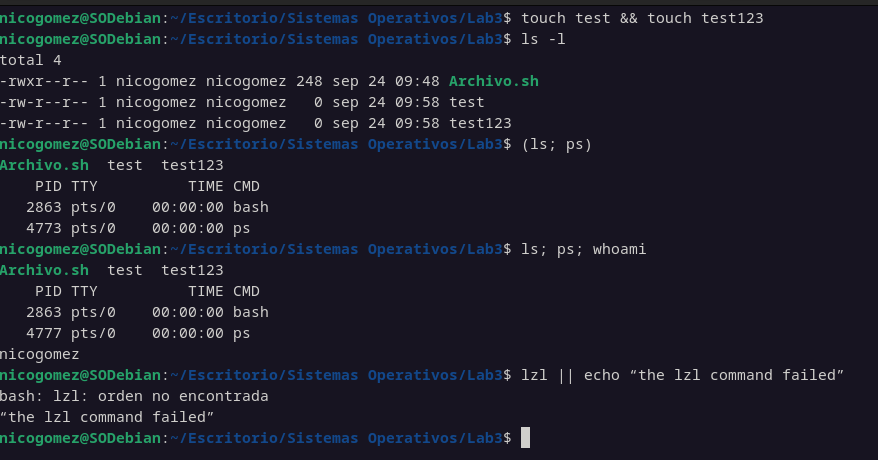
\includegraphics[width=\textwidth]{img/ejerc2.png}
        Como resultado de la ejecución del conjunto de comandos \texttt{touch test \&\& touch test123} se observa que se crean los archivos \textit{test} y \textit{test123}, por otro lado, al ejecutar el conjunto de comandos \texttt{(ls; ps)} se observa que se listan los los procesos en ejecución, para el caso de \texttt{ls; ps; whoami} se observa que se listan los los procesos en ejecución y el usuario actual y finalmente al ejecutar \texttt{lzl || echo "the lzl command failed"} se observa un error del bash ya que el comando \texttt{lzl} no existe, ademas de la impresión del texto \textit{''the lzl command failed''}.
    \end{figure}
    \item Pipe (5pts)
    \begin{figure}[H]
        \centering
        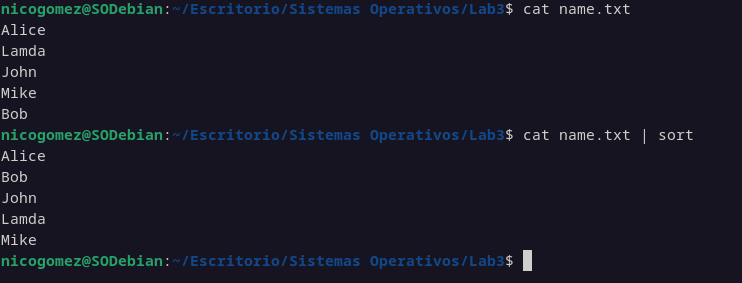
\includegraphics[width=\textwidth]{img/ejerc3.png}
        Para este caso se creo un archivo a parte con de nombre \textit{name.txt} que contiene una lista de 5 nombres, por consiguiente se ejecuta el comando \texttt{cat name.txt | sort} el cual imprime los nombres ordenados alfabéticamente.
    \end{figure}
    \newpage
    \item Redirection (5pts)
    \begin{figure}[H]
        \centering
        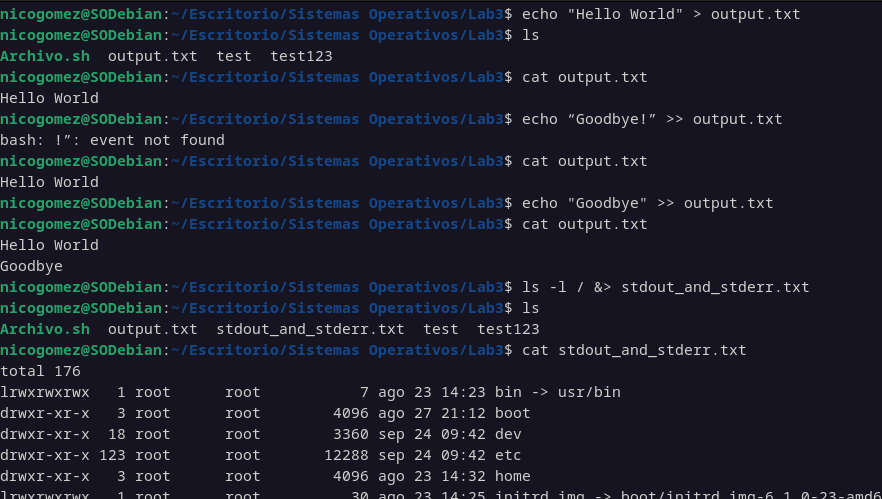
\includegraphics[width=\textwidth]{img/ejerc4.png}
        Para este ejercicio se hizo lo siguiente:
    \end{figure}
\end{enumerate}
\begin{itemize}
    \item Se ejecuto \texttt{echo "Hello World" > output.txt}: Este comando creo un archivo llamado \textit{output.txt} con el contenido \textit{Hello World}.
    \item Se ejecuto \texttt{echo "Goodbye" >> output.txt}: Este comando agrego el contenido \textit{Goodbye} al final del archivo \textit{output.txt}.
    \item Se ejecuto \texttt{cat output.txt}: Este comando imprime el contenido del archivo \textit{output.txt} para ver los cambios realizados.
    \item Se ejecutó \texttt{ls -l / \&> stdout\_and\_stderr.txt}: Este comando imprime el contenido de la lista de archivos del directorio raíz y lo guarda en el archivo \textit{stdout\_and\_stderr.txt}.
\end{itemize}

\newpage
\subsection*{Parte B}
\begin{figure}[H]
    \centering 
    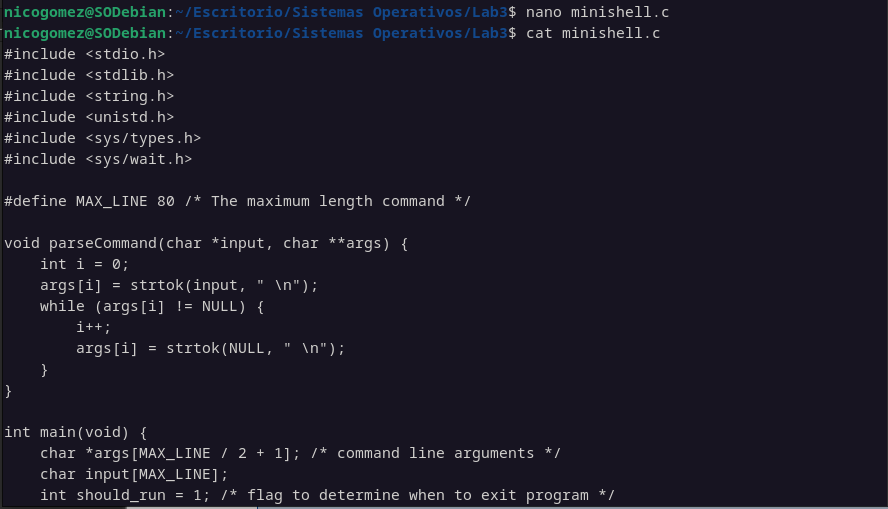
\includegraphics[width=0.65\textwidth]{img/ejerc5part1.png}
    \\Se creo el archivo \textit{minishell.c} en el cual se introdujo la secuencia de comandos asignada. 
\end{figure}
\begin{figure}[H]
    \centering
    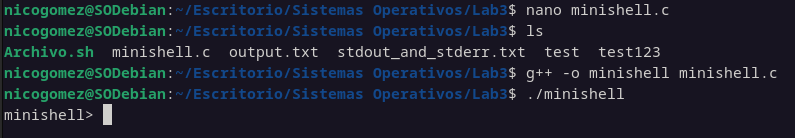
\includegraphics[width=\textwidth]{img/ejerc5part2.png}
    \\Se ejecuto el archivo \textit{minishell.c}.
\end{figure}
\begin{enumerate}
    \newpage
    \item Ejecuta comandos básicos como ‘ls’, ’pwd’, ’date’. Luego prueba la redirección de entrada y salida ‘ls > output.txt’, ‘sort < file.txt > sorted.txt’ y ejecuta comandos en segundo plano ‘sleep 10 \&’. Explica lo sucedido. (15pts)
    \begin{figure}[H]
        \centering
        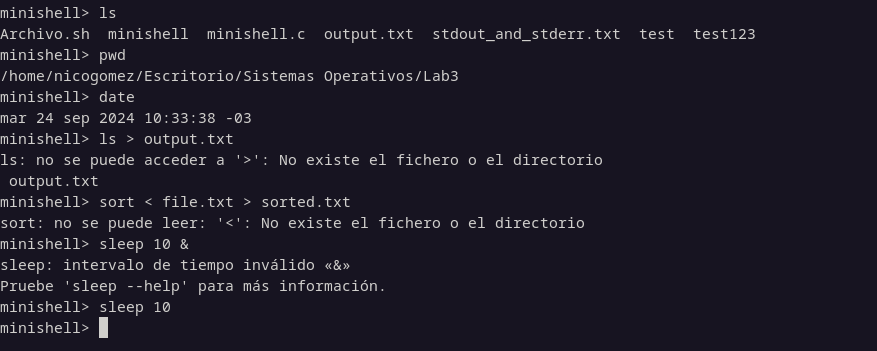
\includegraphics[width=\textwidth]{img/ejerc5part3.png}
        Se ejecutó el comando \texttt{ls} el cual me listó los archivos y carpetas existentes, se ejecutó el comando \texttt{pwd} el cual me muestra la ruta actual, se ejecutó el comando \texttt{date} el cual me muestra la fecha y hora actual, se ejecutó el comando \texttt{ls > output.txt} el cual me lanzó el error \textbf{ls: no se puede acceder a '>': No existe el fichero o el directorio} siendo que el archivo \textit{output.txt} sí existe por lo que el error se puede deber a que el comando general del minishell no está diseñado para esta funcionalidad, se ejecutó el comando \texttt{sort < file.txt > sorted.txt} el cual también me lanzó el error \textbf{sort: no se puede leer '<': No existe el fichero o el directorio} sin embargo para este caso nunca existió el archivo \textit{file.txt} por lo que el error se debe a que el archivo no existe, por último se ejecutó el comando \texttt{sleep 10 \&} el cual me lanzó el error \textbf{bash: error sintáctico cerca del elemento inesperado `\&'} el cual se debe a que el comando no está bien estructurado pero al ejecutar el comando \texttt{sleep 10 \&} sí se ejecuta correctamente.
    \end{figure}
    \item Investiga y añade soporte para el comando ‘cd’. Copia tu código completo aquí. (40pts)
\end{enumerate}

\begin{figure}[H]
    \centering
    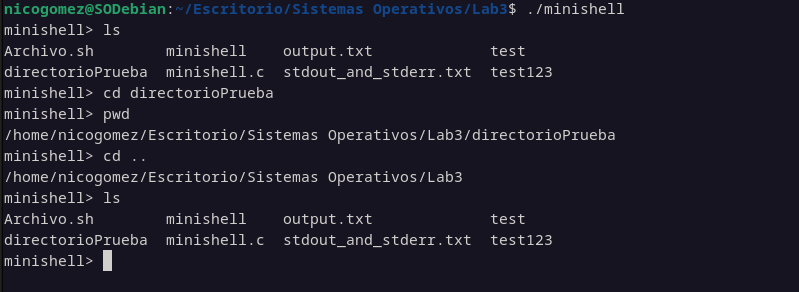
\includegraphics[width=\textwidth]{img/ejerc5part4.png}
    \\Se añadió soporte para el comando \texttt{cd} en el archivo \textit{minishell.c}.
\end{figure}
\begin{figure}[H]
    \centering
    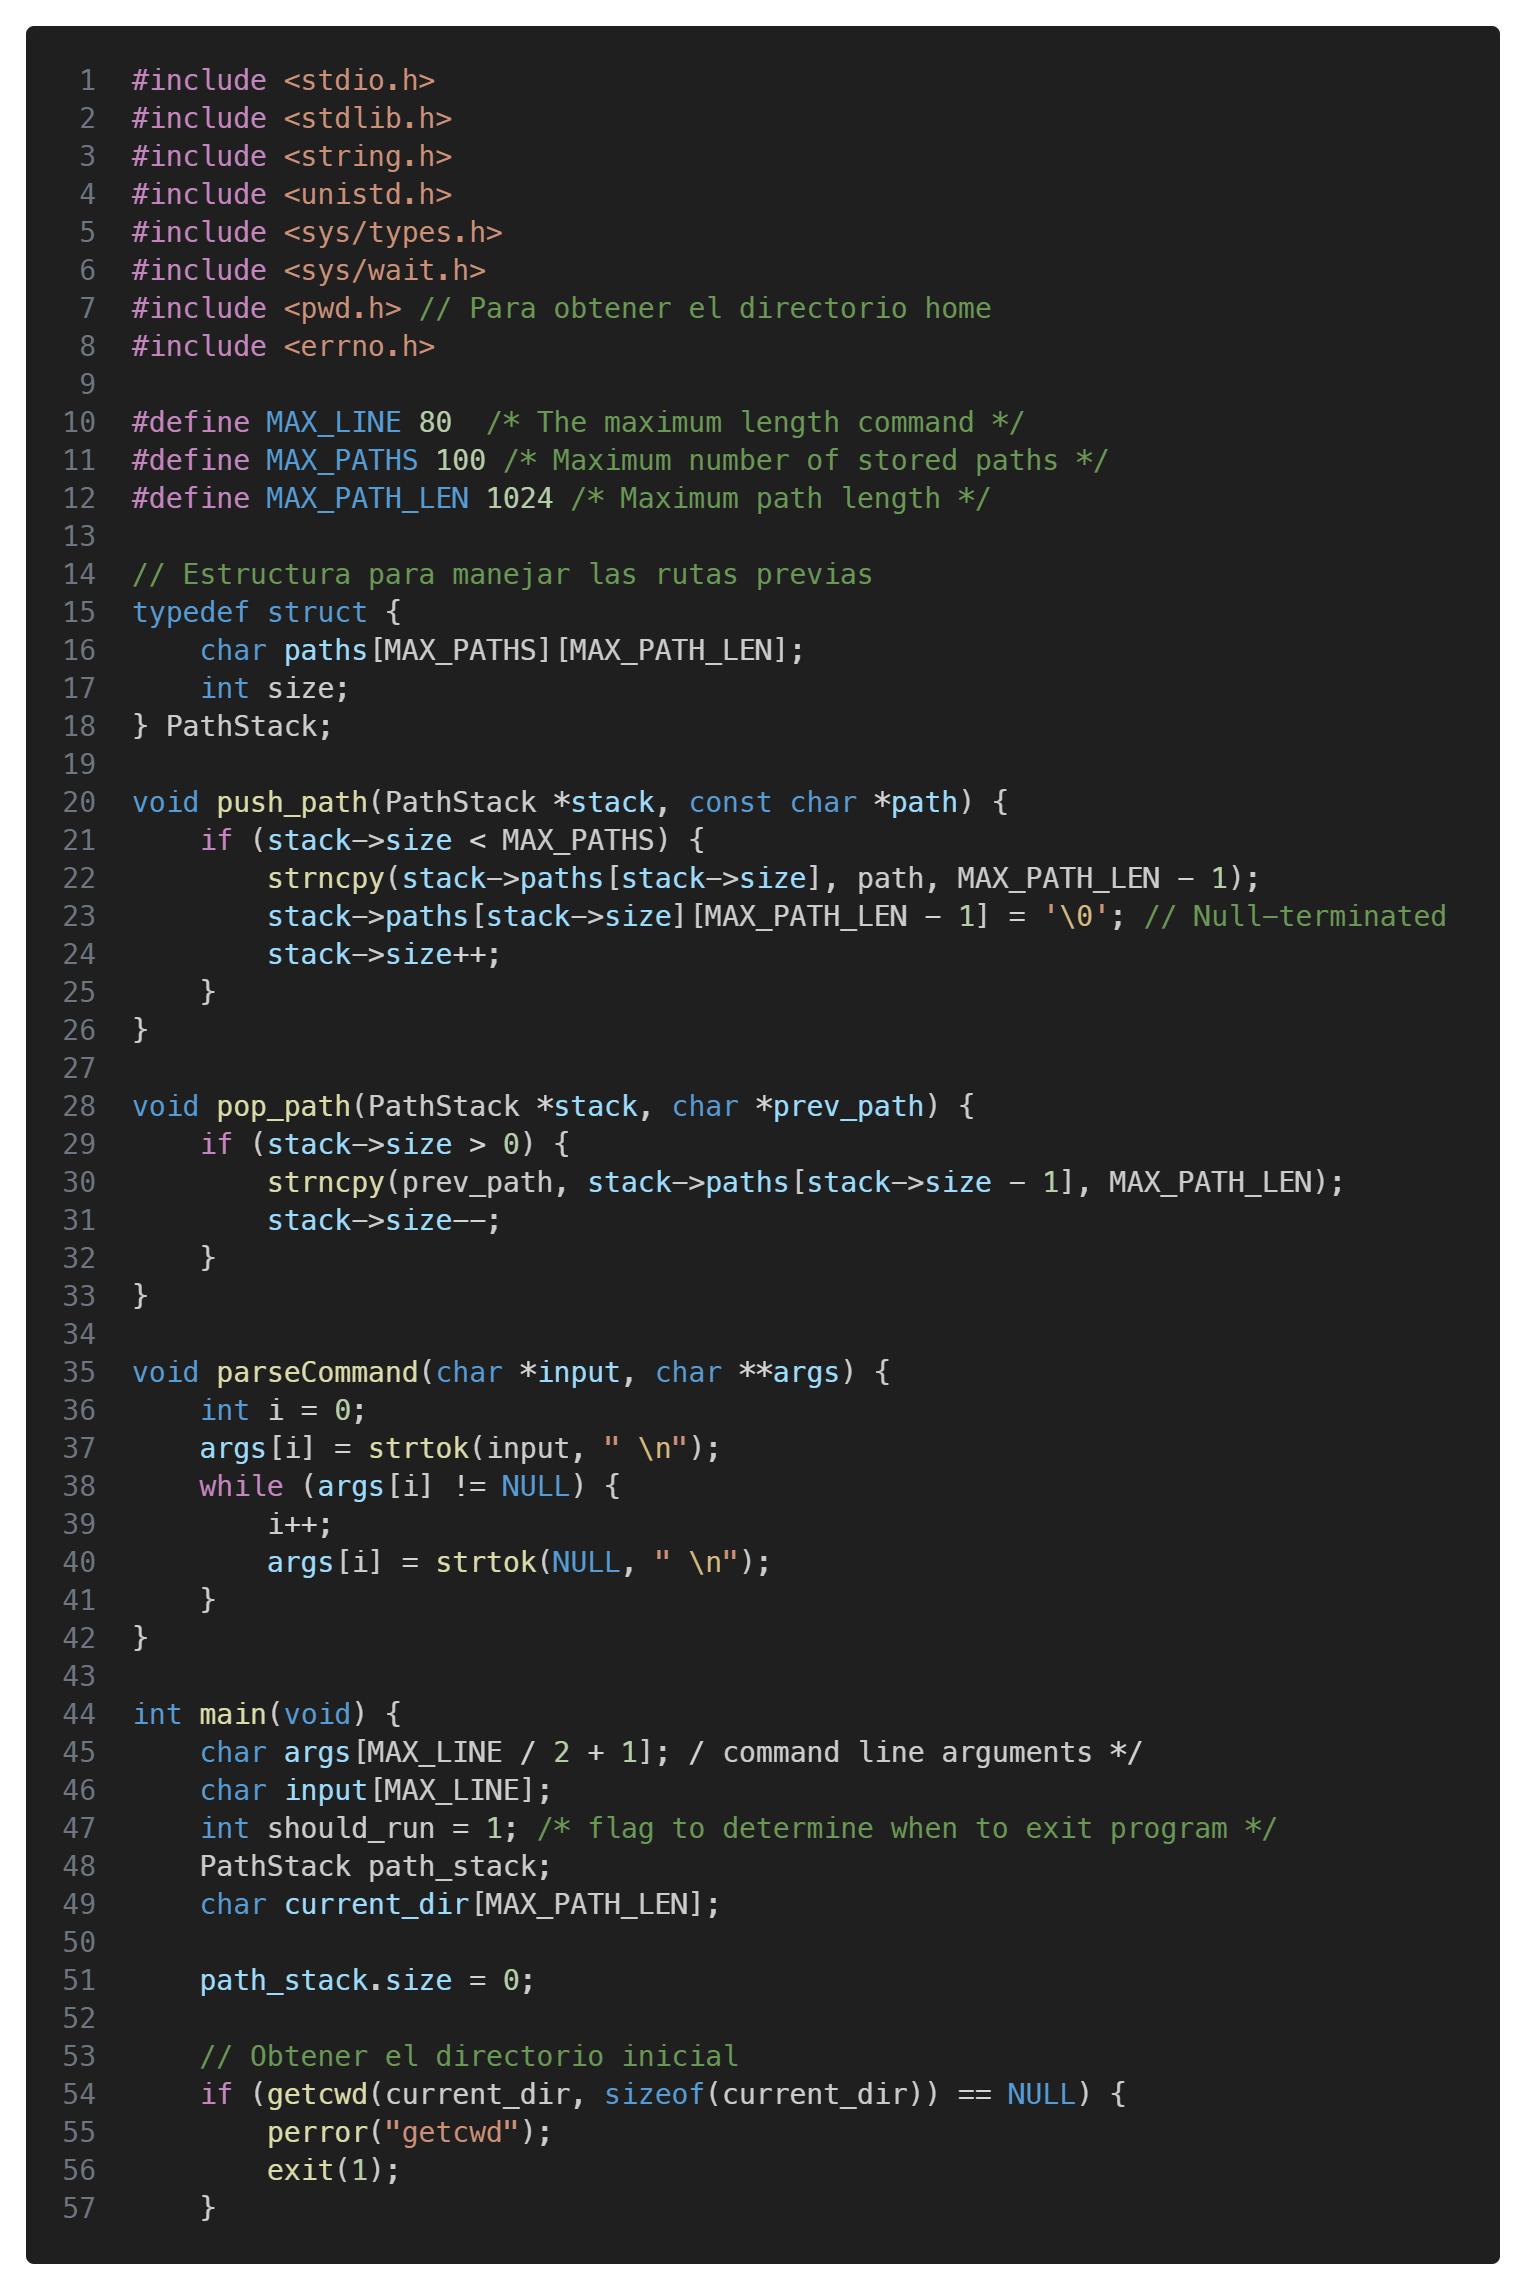
\includegraphics[width=\textwidth]{img/code1.png}
\end{figure}
\begin{figure}[H]
    \centering
    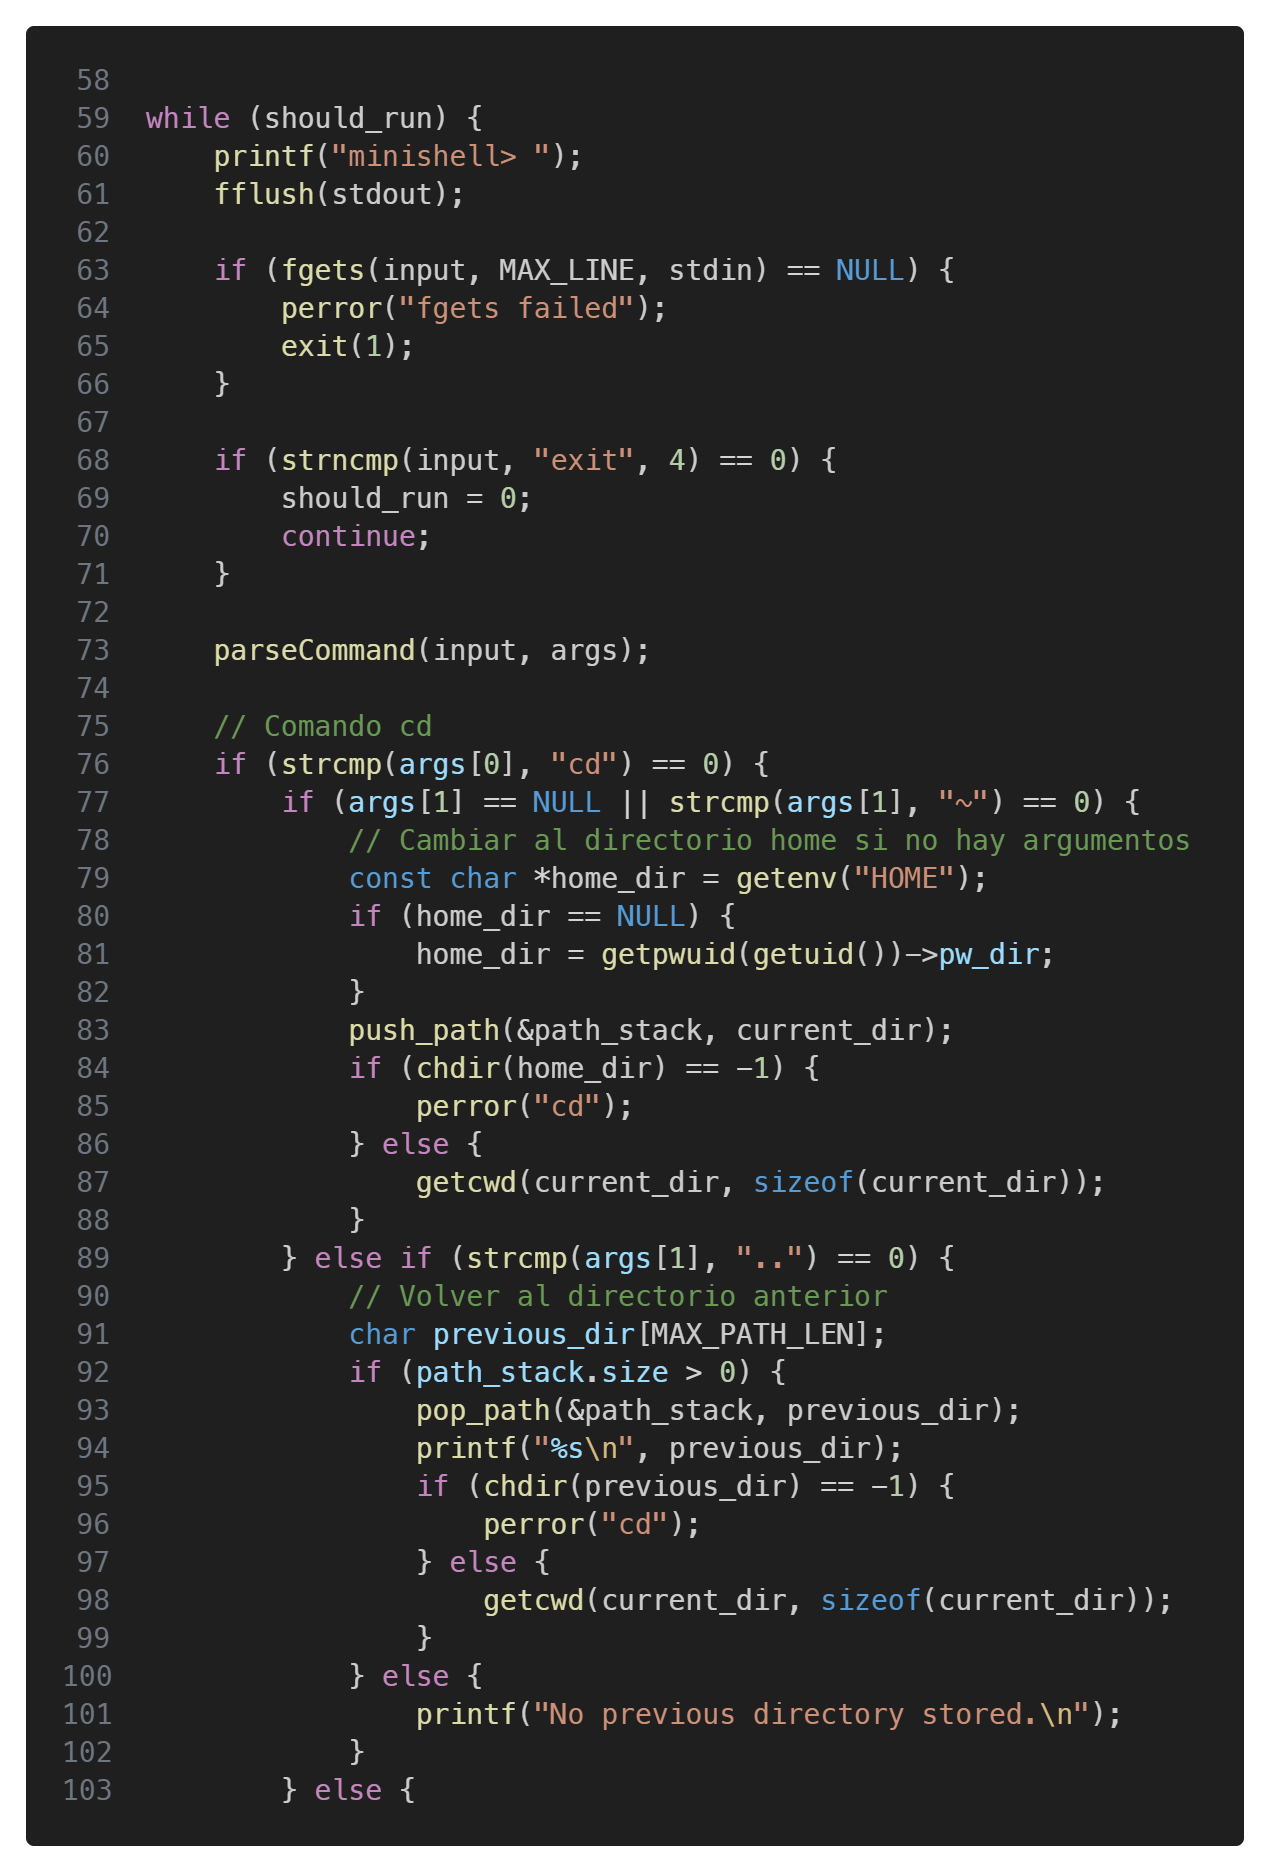
\includegraphics[width=\textwidth]{img/code2.png}
\end{figure}
\begin{figure}[H]
    \centering
    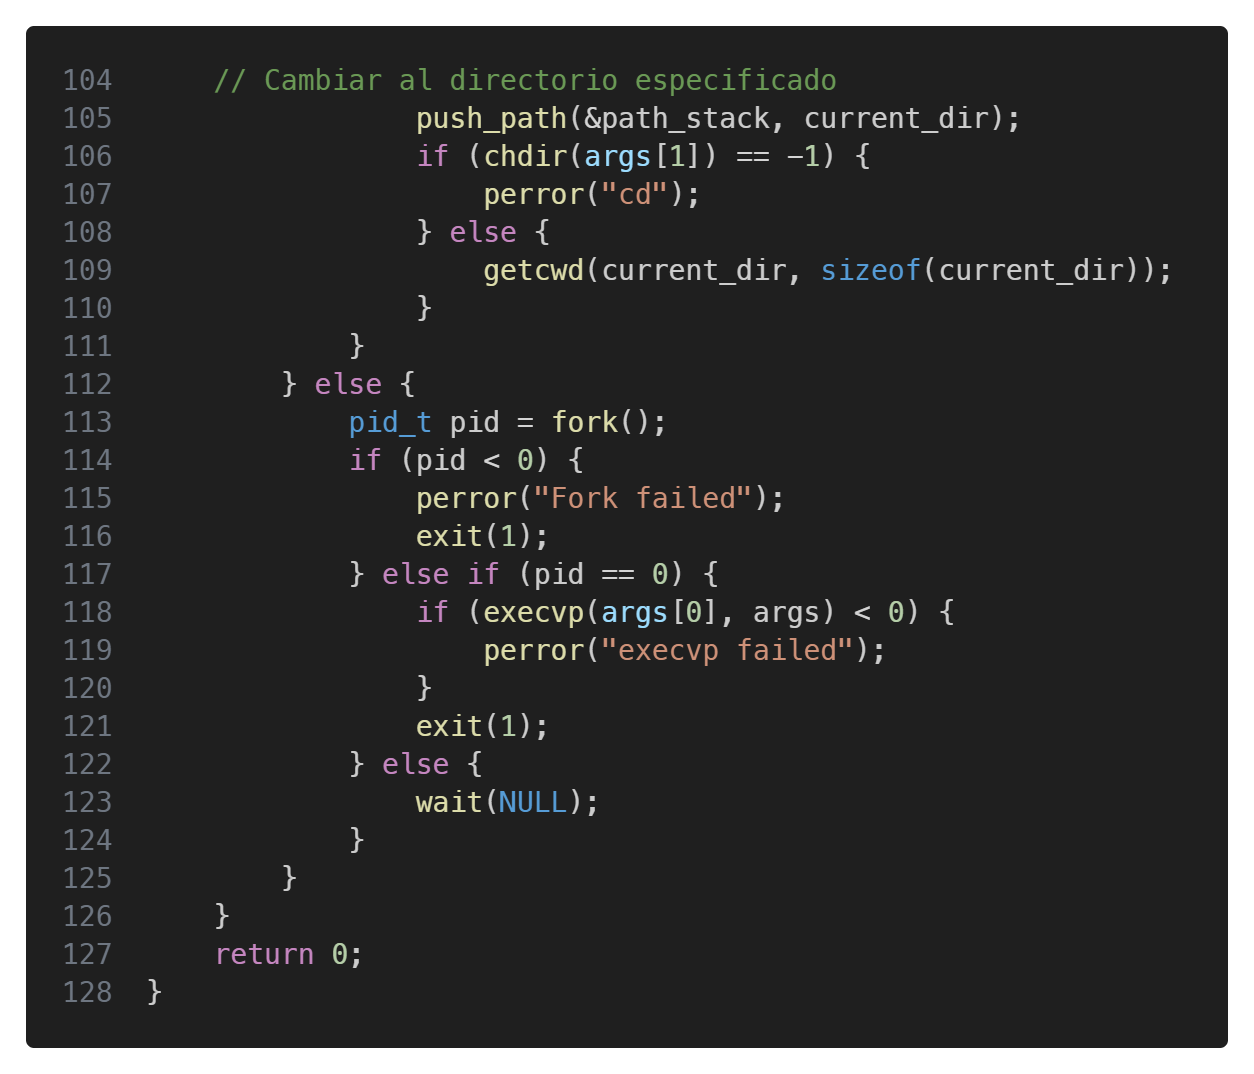
\includegraphics[width=\textwidth]{img/code3.png}
\end{figure}

\end{document}